
\RequirePackage{silence} % :-\
%    \WarningFilter{scrreprt}{Usage of package `titlesec'}
%    \WarningFilter{scrreprt}{Activating an ugly workaround}
%    \WarningFilter{titlesec}{Non standard sectioning command detected}
\documentclass[ twoside,openright,titlepage,numbers=noenddot,%1headlines,
headinclude,footinclude,cleardoublepage=empty,abstract=on,
BCOR=5mm,paper=a4,fontsize=11pt, dvipsnames
]{scrreprt}
\usepackage{todonotes}
\usepackage{xspace}
\usepackage{minted}
\PassOptionsToPackage{utf8}{inputenc}
\usepackage[pdfusetitle]{hyperref}
\usepackage{inputenc}
\PassOptionsToPackage{T1}{fontenc} % T2A for cyrillics
\usepackage{fontenc}

\PassOptionsToPackage{
%  drafting=false,    % print version information on the bottom of the pages
  tocaligned=false, % the left column of the toc will be aligned (no indentation)
  dottedtoc=false,  % page numbers in ToC flushed right
  eulerchapternumbers=true, % use AMS Euler for chapter font (otherwise Palatino)
  linedheaders=false,       % chaper headers will have line above and beneath
  floatperchapter=true,     % numbering per chapter for all floats (i.e., Figure 1.1)
  eulermath=false,  % use awesome Euler fonts for mathematical formulae (only with pdfLaTeX)
  beramono=false,    % toggle a nice monospaced font (w/ bold)
  palatino=false,    % deactivate standard font for loading another one, see the last section at the end of this file for suggestions
  style=classicthesis % classicthesis, arsclassica
}{classicthesis}

\makeatletter
\DeclareFixedFont{\chapterNumber}{U}{eur}{b}{n}{20}
\DeclareFixedFont{\chapterNumber}{T1}{pplj}{m}{n}{20}
\makeatother
\usepackage{amsmath,amssymb}
\usepackage{mathtools}

\newcommand{\myTitle}{Complex fluids in the GPU era\xspace}
\newcommand{\mySubtitle}{Algorithms and simulations\xspace}
\newcommand{\myDegree}{\xspace}
\newcommand{\myName}{Ra\'ul P. Pel\'aez\xspace}
\newcommand{\myProf}{Rafael Delgado Buscalioni\xspace}
\newcommand{\myOtherProf}{\xspace}
\newcommand{\mySupervisor}{\xspace}
\newcommand{\myFaculty}{Facultad de Ciencias\xspace}
\newcommand{\myDepartment}{Departamento de F\'isica Te\'orica de la Materia Condensada\xspace}
\newcommand{\myUni}{Universidad Aut\'onoma de Madrid\xspace}
\newcommand{\myLocation}{\xspace}
\newcommand{\myTime}{2022\xspace}
\newcommand{\myVersion}{v1.0}
\PassOptionsToPackage{american}{babel}
\usepackage{babel}
\usepackage{doi}
\usepackage{csquotes}
\PassOptionsToPackage{%
  %backend=biber,bibencoding=utf8, %instead of bibtex
  backend=bibtex8,bibencoding=ascii,%
  language=auto,%
  style=numeric-comp,%
  eprint=false,
  %style=authoryear-comp, % Author 1999, 2010
  %bibstyle=authoryear,dashed=false, % dashed: substitute rep. author with ---
  sorting=none,
  maxbibnames=3, % default: 3, et al.
  %backref=true,%
  doi=true,
  url=false,
  natbib=true % natbib compatibility mode (\citep and \citet still work)
  }{biblatex}
\usepackage{biblatex}       

%\PassOptionsToPackage{fleqn}{amsmath}       % math environments and more by the AMS

\usepackage{graphicx}
\usepackage{scrhack} % fix warnings when using KOMA with listings package
\usepackage{xspace} % to get the spacing after macros right

\usepackage{tabularx} % better tables
\setlength{\extrarowheight}{3pt} % increase table row height
\usepackage{listings}
\usepackage{classicthesis}
\makeatletter
\AtBeginDocument{
\hypersetup{%
%  %draft, % hyperref's draft mode, for printing see below
  colorlinks=true
  %, linktocpage=true, pdfstartpage=3, pdfstartview=FitV,%
%  % uncomment the following line if you want to have black links (e.g., for printing)
   %colorlinks=false, linktocpage=false, pdfstartpage=3, pdfstartview=FitV, pdfborder={0 0 0},%
%  breaklinks=true, pageanchor=true,%
%  pdfpagemode=UseNone, %
%  % pdfpagemode=UseOutlines,%
%  plainpages=false, bookmarksnumbered, bookmarksopen=true, bookmarksopenlevel=1,%
%  hypertexnames=true, pdfhighlight=/O,%nesting=true,%frenchlinks,%
%  urlcolor=CTurl, linkcolor=CTlink, citecolor=CTcitation, %pagecolor=RoyalBlue,%
%  %urlcolor=Black, linkcolor=Black, citecolor=Black, %pagecolor=Black,%
%  pdfpagelabels=true,
  pdftitle={Complex fluids in the GPU era},        
  pdfauthor={\textcopyright\ \myName, \myUni, \myFaculty},%
%  pdfsubject={Complex fluids, GPUs},%
%  pdfkeywords={},%
  pdfcreator={pdfLaTeX},%
  pdfproducer={LaTeX with hyperref and classicthesis}%
}
}
\makeatother


% Changing the text area
%\areaset[current]{312pt}{761pt} % 686 (factor 2.2) + 33 head + 42 head \the\footskip
%\setlength{\marginparwidth}{7em}%
%\setlength{\marginparsep}{2em}%


\usepackage{amsmath}
\usepackage{algorithm}
\usepackage{algpseudocode}
\algnewcommand{\LeftComment}[1]{\Statex \(\triangleright\) #1}
\algnewcommand{\Input}[1]{\hspace*{\algorithmicindent} \textbf{Input:} #1}
\usepackage{bm}
\usepackage{hyperref}
\usepackage[acronym]{glossaries}
\usepackage[utf8]{inputenc}
\usepackage{pgfplots}
\graphicspath{{./gfx/}}

\newcommand{\executeiffilenewer}[3]{
  \ifnum
  \pdfstrcmp{\pdffilemoddate{#1}}{\pdffilemoddate{#2}}>0
  {\immediate\write18{#3}}
  \fi
}
\newcommand{\includesvg}[2]{
  \executeiffilenewer{#1.svg}{#1.pdf}
  {inkscape -D #1.svg --export-type=pdf } %  --export-latex}
  %\def\svgwidth{#2}
  % \input{#1.pdf_tex}
  \includegraphics[width=#2]{#1.pdf}
}

\makeglossaries
\newacronym{UAMMD}{UAMMD}{Universaly Adaptable Multiscale Molecular Dynamics}
\newacronym{MD}{MD}{Molecular Dynamics}
\newacronym{BD}{BD}{Brownian Dynamics}
\newacronym{BDHI}{BDHI}{Brownian Dynamics with Hydrodynamic Interactions}
\newacronym{IBM}{IBM}{Immersed Boundary}
\newacronym{PSE}{PSE}{Positively Split Ewald}
\newacronym{FCM}{FCM}{Force Coupling Method}
\newacronym{ICM}{ICM}{Inertial Coupling Method}
\newacronym{FIB}{FIB}{Fluctuating Immersed Boundary}
\newacronym{DPD}{DPD}{Dissipative Particle Dynamics}
\newacronym{SPH}{SPH}{Smoothed Particle Hydrodynamics}
\newacronym{SE}{SE}{Spectral Ewald}
\newacronym{LJ}{LJ}{Lennard-Jones}
\newacronym{MIC}{MIC}{Minimum Image Convention}
\newacronym{FFT}{FFT}{Fast Fourier Transform}
\newacronym{iFFT}{iFFT}{Inverse Fast Fourier Transform}
\newacronym{GPU}{GPU}{Graphical Processor Units}
\newacronym{GPGPU}{GPGPU}{General Purpose Computing on GPU}
\newacronym{RHS}{RHS}{Right Hand Side}\newcommand{\rhs}{\gls{RHS}\xspace}
\newacronym{API}{API}{Application Programming Interface}
\newacronym{BVP}{BVP}{Boundary Value Problem} \newcommand{\bvp}{\gls{BVP}\xspace}
\newacronym{BC}{BC}{Boundary Condition} \newcommand{\bc}{\gls{BC}\xspace}\newcommand{\bcs}{\gls{BC}s\xspace}


\renewcommand{\vec}[1]{\bm{#1}}
\newcommand{\uammd}{\gls{UAMMD}\xspace}
\newcommand{\gpu}{\gls{GPU}\xspace}
\newcommand{\dt}{\delta t}
\newcommand{\half}{\frac{1}{2}}
\newcommand{\red}[1]{{\color{red}#1}}
\DeclareMathOperator{\erf}{erf}


\addbibresource{Bibliography.bib}

%\hyphenation{put special hyphenation here}

\begin{document}
\frenchspacing
\raggedbottom
\selectlanguage{american} % american ngerman
%\renewcommand*{\bibname}{new name}
%\setbibpreamble{}
\pagenumbering{roman}
\pagestyle{plain}

\input{FrontBackmatter/DirtyTitlepage}
\input{FrontBackmatter/Titlepage}
\input{FrontBackmatter/Titleback}
\cleardoublepage%*******************************************************
% Dedication
%*******************************************************
\thispagestyle{empty}
\phantomsection
\pdfbookmark[1]{Dedication}{Dedication}

\vspace*{3cm}

\begin{center}
      This thing is complex... so complex not even God gets it.\\ \medskip
    --- Rafa Buscalioni
    \\ \medskip\medskip
        There is no way you are getting a quote for your stupid thesis\\ \medskip
    --- NVIDIA

\end{center}

\medskip

%\cleardoublepage\input{FrontBackmatter/Foreword}
\cleardoublepage%*******************************************************
% Abstract
%*******************************************************
%\renewcommand{\abstractname}{Abstract}
\pdfbookmark[1]{Abstract}{Abstract}
% \addcontentsline{toc}{chapter}{\tocEntry{Abstract}}
\begingroup
\let\cleardoublepage\relax
\let\cleardoublepage\relax
\let\cleardoublepage\relax

\chapter*{Abstract}

Some abstract


\cleardoublepage\input{FrontBackmatter/Publications}
\cleardoublepage%*******************************************************
% Acknowledgments
%*******************************************************
\pdfbookmark[1]{Acknowledgments}{acknowledgments}

\begin{flushright}{\slshape}
\end{flushright}



\bigskip

\begingroup
\let\clearpage\relax
\let\cleardoublepage\relax
\let\cleardoublepage\relax
\chapter*{Acknowledgments}

\cleardoublepage\input{FrontBackmatter/Contents}

\cleardoublepage
\pagestyle{scrheadings}
\pagenumbering{arabic}
%\setcounter{page}{90}
% use \cleardoublepage here to avoid problems with pdfbookmark
\cleardoublepage
\part{Introduction}\label{pt:intro}
\chapter{Introduction}\label{ch:introduction}


The modeling and simulation of physical systems is always tied to a certain spatio-temporal scale. More often than not, studying a system through the lens of a certain scale prevents the exploration of the others.
Choosing the right lens for a problem requires understanding of its characteristic times and lengths.
Say, for instance, that you want to study the caudal of a waterfall throughout the next thousand years. It would be a bad decision to employ quantum mechanics for such a feat, a theoretical framework best suited for events that take femtoseconds and are measured in angstroms.
A lot of mathematical frameworks and numerical techniques are known for the exploration of different spatio-temporal scales. However, some times the need arises to tackle a phenomenon that unravels between their scope.
On the other hand, the advent of supercomputing in the last two decades has presented the field with new powerful tools to leverage. For the first time we have more computing power than what our techniques are capable of handling. 
Developing new techniques (numerical and theoretical) directly aimed to these new techonologies will allow to explore regimes previously unreachable, opening the doors to a world of secrets waiting to be found.
The fields that can take advantage of more computing power the most are those that mix several spatio-temporal regimes.
For instance, when we need to simulate every molecule of a virus capsid submerged in water for a very long time\cite{virusfullatom2018}. In this article, the authors simulate the dynamics of $6$ million atoms (explicitly) in the span of $1\mu s$, requiring $5 10^8$ simulation steps.
Of course, this kind of simulation would be impossible without the aid of a super computer and a family of software tools to take advantage of it.
This thesis is devoted to the development of new algorithms and software tools for the study of complex fluids and biological systemsin high performance computing environments. It just so happens that the interesting physics of these processes often lie in this intermediate regime, called the \emph{mesoscale}.
The definition of mesoscale is kind of fuzzy, but mesoscopic physics normally deal with entities ranging from $50-100nm$ (a typical virus) to $~10\mu m$ (the size of a HeLa cell), with characteristic times going from a few micro seconds to even minutes.
The mesoscale poses a series of theoretical and numerical challenges, stemming from the wide range of spatio-temporal scales that influence them. A perfect fit for a super computer.
Another example of this kind of simulations is the one described in \cite{fullatombacteria2016}. In this article the authors employ $100$ million particles to simulate a chunk of the interior environment of a bacteria for some tens of nanoseconds (around $10^7$ steps).

Recently, a new paradigm of supercomputing has arisen. The \gpu, a massively parallel copocressor. So powerful that it requires to straight-up rethink our algorithms to take advantage of it.

\begin{figure}
  \label{fig:landscape}
  \centering
%  \begin{tikzpicture}
%    \begin{loglogaxis}[
%      width=\textwidth,
%      height=\axisdefaultheight,
%      xmin=1e-11,xmax=100,
%      xtick={1e-10, 10e-9, 1e-6, 1e-3, 1, 100},
%      xticklabels={0.1 nm, 10 nm, 1 $\mu$m, 1 mm, 1 m, 100 m},
%      ymin=1e-15,ymax=86400,
%      ytick={1e-15, 1e-12, 1e-9, 1e-6, 1e-3, 1, 3600, 86400},
%      yticklabels={1 fs, 1 ps, 1 ns, 1 $\mu$s, 1 ms, 1 s, 1 h, 1 day}
%      ]
%      \addplot[color=red, domain=1e-11:100 ]{1000000*x^2.5};
%    \end{loglogaxis}
%  \end{tikzpicture}
  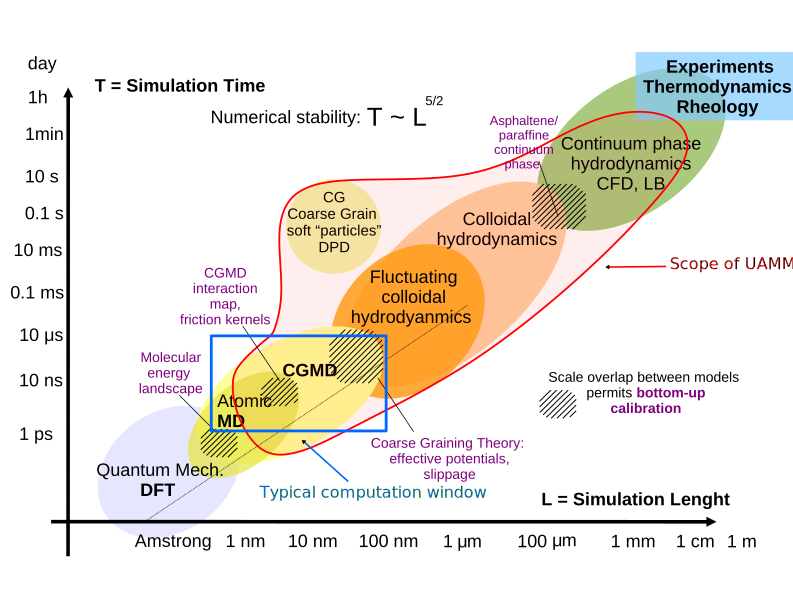
\includegraphics[width=\textwidth]{landscape}
  \caption{A landscape of numerical techniques}
\end{figure}

\section{The Graphical Processor Unit}

The \gpu technology, interpreted as some kind of specialized graphic circuit or co-processor, can be tracked back to the 1970s. Once electronic devices started having screens attached to them, it made sense to have some kind of chip translating the CPU information into the analogic signal of the display. It was then only a matter of time before more functionality was put into them. It started as a way to accelerate the display process in early video game hardware, such as arcade systems.
Storing the data that goes into the screen takes a lot of space and, at the time, RAM memory was expensive (still is, by the way!).

In 1977, the Atari 2600 (one of the first home consoles) could simply not afford to store the contents of its 160x80 pixel display into its 128 bytes of RAM. Of course, these systems employed some truly creative software tricks to reduce memory usage. However, the numbers just do not add up. Even if we limit ourselves to a monochrome output (so one pixel takes one bit to store), the frame buffer for a 160x80 pixel display takes 1600 bytes\footnote{In contrast, the NVIDIA GTX 980 (the trusty, consumer-grade, GPU that has accompanied my thoughout most of my Ph.D.) has 4 GB of memory and will happily output to a several screens with 4k resolution (4096x2160 pixels).}.
The solution was to not have a frame buffer at all, rather outsource the display operations to a specialized hardware. The Atari 2600's graphic chip had a 128 color palette and allowed developers to use close to 5 sprites to design their 2D games.

These chips were little more than video display chips, but they were the predecesors to the \gpu.
Throughout the next decade the hardware evolves to support faster and more complex operations, hold more memory, etc. In 1990 a graphic adaptor could draw 16 million different colors to a 1028x1024 pixel display and hold 1MB of data.

Graphic adaptors were still centered around 2D graphic acceleration, such as graphical user interfaces and 2D games. However, the market was already pushing for real-time 3D graphics in games. Although one could hack the current 2D graphic pipeline to draw 3D environments, without specialized hardware acceleration (as was already common for 2D) the results were far from interactive. Surely it would be a task best suited for the graphic adaptor technology already established.

Soon enough, during the early and mid 1990s, several companies were releasing their graphic adaptors with 3D acceleration capabilities. In 1994 the term \gpu is coined to designate this hardware, which had evolved beyond its original task of just sending pixels to a display.
OpenGL\cite{opengl}, one of the first graphics \gls{API}\footnote{A software library.}, appears in the early 1990s attempting to standardize the programming of graphic hardware accelerators, specially for 3D.
At the time OpenGL had quite limited capabilities, allowing a developer to do little more than to feed a fixed pipeline with triangles. OpenGL would then interface with the \gpu to turn this geometry into a 2D image that could be displayed.
Naturally this translation involves a great deal of raw computation, further transforming the \gpu from a video display card to an independent co processor. Furthermore the usual operations required to do this happen to be inherently parallel. While the CPU evolved to be formed by a single, powerful, core the \gpu was born out of a parallel computing necessity. Thus a \gpu tends to have many, less powerful, processing cores.
Jumping again to the year 2000 the quality and complexity of computer graphics has exploded. Card manufacturers have included all sorts of new 3D hardware accelerated operations beyond simple triangles. And OpenGL has evolved along them. As it usually happens people have started to hack around, using the graphics pipeline to perform computations not necessarily related to computer graphics. In particular, a new \gpu was presented by the NVIDIA Corporation in 2001 that allowed to modify the different stages of the graphic pipeline via something called programmable shaders. These shaders were short programs that could intercede between the different stages of drawing. A vertex shader could be written to process each triangle before sending it to a fragment shader, which could process each pixel on the screen before finally sending them to the display. This was the advent of the so-called \gls{GPGPU}.

Shaders were enough for the community to realize that drawing polygons was far from the only thing they could do with a \gpu\cite{gpgpu2002}. Applications exploting shaders arise everywhere in a variety fields like scientific image processing \cite{gpuimage2003, gpuimage2006}, lineal algebra \cite{gpulinalg2001, gpulinalg2003a, gpulinalg2003b}, physics \cite{gpulbm2004} and even machine learning\cite{gpuml2005, gpuml1998}. One can even find a molecular dynamics code running on the \gpu of a Sony PlayStation 3 \cite{ps3md2009}.

The next natural step took place in 2007, when the NVIDIA Corporation released CUDA\cite{cuda}.
\begin{figure}
  \centering
  \includegraphics[width=\textwidth]{gpu_and_me}
  \caption{A picture of the author with a GPU ( a NVIDIA's RTX 2080Ti ).}
  \label{fig:gpuandme}
\end{figure}

\section{Software for soft matter simulations}
Problems with porting CPU centric \gls{MD} packages to \gpu. Scalability in software.

Many \gls{MD} software projects started at a time when the \gpu was not a widespread tool for general computing (or did not even existed as hardware). Take for example GROMACS \cite{gromacs}, which was born in 1991

The present and future of high performance computing.
CUDA vs alternatives.

Scientific computing in the GPU era.

Developing algorithms for the ground up with the GPU architecture in mind is essential. Leverage ultra efficient \gpu \gls{FFT} by developing spectral algorithms. Many times simplicity beats complexity.

State of the art in molecular simulations.

\cleardoublepage
\ctparttext{Description of the UAMMD infrastructure. Importance of fundamentally GPU-driven design.}
\part{UAMMD: Design and components}\label{pt:uammd}
%*****************************************
\chapter{Design principles}\label{ch:design}
Open infrastructure instead of closed ecosystem. Open source. C++, header only.
\section{Universality}
Anything goes as long as it has interacting entities. One could technically implement Chess as a module.
\section{Adaptability}
Highly templated code and super generic interfaces. 
\section{Mulstiscale}
From atoms in vacuum to chunks of oceans and planetary dynamics.
\section{Molecular Dynamics}
Using molecular in the sense of an arbitrarily coarsed-grained simulation unit (atoms, groups of atoms, colloids, groups of colloids, buckets of water, planets...)

\chapter{Core Components}\label{ch:core}
How the design principles are exposed in code.
\section{System}
\section{ParticleData}

\section{ParticleGroup} 




\chapter{Algorithms}\label{ch:algorithms}
Algorithms in the basic \gls{UAMMD} infrastructure. 
\section{Cell List}
No need to really construct a neighbour list, reference  to Transverser
\section{Verlet List}
mostly obsolete thanks to cell list
\section{Bonded Forces}
Bonded Forces as a kind of neighbour list
\section{IBM}\label{ch:ibm}
Change to something more meaningful that conveys spreading+interpolation


\chapter{Interfaces}\label{ch:interfaces}
This stuff should go organically in the text
Generic interfaces desgined to communicate with the core \gls{UAMMD} componentes.
\section{Transverser}
The Transverser interface. Transform + traverse
\section{Potential}
To encapsulate Transversers
\section{ParameterUpdatable}
An interface to communicate changes in parameters


\section{Usage examples throughout this document}\label{sec:uammd_struct}
Every time an algorithm available in \uammd is presented it will be acompanied by a section describing how to use it in the codebase.
Often this will consist of a function creating and returning an instance of the related module in the following form


\begin{minted}{c++}
#include<uammd.cuh>
//Additional includes when necessary
using namespace uammd;
auto createModule(UAMMD sim){
//Some preparation...
return std::make_shared(Module(/*Whatever is needed*/));
}
\end{minted}

These examples are meant to serve both as a tutorial and an easily copy-pastable example.
The structure \emph{UAMMD} in these examples is not part of \uammd and is meant to group the core components of a typical \uammd code. It can be defined as follows


\begin{minted}{c++}
#include<uammd.cuh>
//Additional includes when necessary
using namespace uammd;
//An aggregate of parameters required by the relevant modules in the code
struct Parameters{
  //real dt;
  //...
};
struct UAMMD{
  std::shared_ptr<System> sys;
  std::shared_ptr<ParticleData> pd;
  std::shared_ptr<ParticleGroup> pg;
  Parameters par;
};

//A function creating an instance of the UAMMD structure
UAMMD initializeUAMMD(){
  UAMMD sim;
  Parameters par;
  //Fill out parameters somehow
  //par.dt = 0.1;
  sim.par = par;
  sim.sys = std::make_shared<System>();
  //Set the number of particles some how.
  int numberParticles = 1e6;
  sim.pd  = std::make_shared<ParticleData>(sys, numberParticles);
  //A group with all the particles.
  sim.pg = std::make_shared<ParticleGroup>(pg, sys, "All");
  return sim;
}
\end{minted}

\section{Error handling in UAMMD}\label{sec:uammd_errors}
Errors are communicated via C++ exceptions.


\section{Basic concepts of GPU programming}
Things to explain here:

Different memories; Separation between CPU and GPU RAM, global memory, register memory, shared memory, constant memory.

\part{A voyage through numerical space-time}

Let us go through the different numerical techniques that are used to simulate the different sections of the spatio-temporal landscape.

\begin{figure}
  \centering
  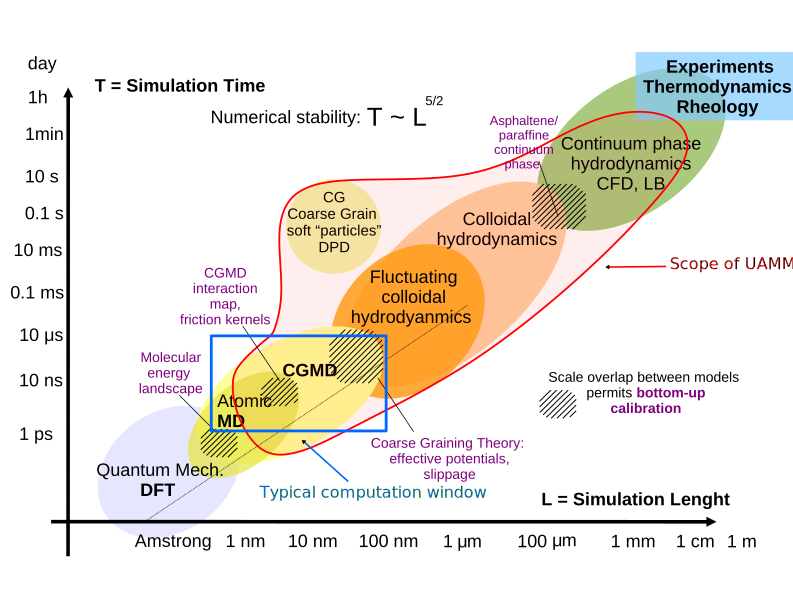
\includegraphics[width=\textwidth]{landscape}
  \caption{The spatio-temporal landscape and its numerical techniques.}
  \label{fig:sptime-land}
\end{figure}


We can distinguish between two families of numerical techniques, particle and grid based methods. The second one also uses particles, but the heavyweight of the algorithm is carried out in a grid, as apposed to just the positions of the particles.
In some way or another, all algorithms have to take into account interactions between particles.

\chapter{Working with particles}
Let us interpret the word \emph{particle} as a relatively small discrete portion in a simulation. This is a vage definition on porpuse, since from an algorithmic point of view it does not really matter what a particle represents. Sometimes a particle will be an atom or molecule, other times it will make more sense that our simulation unit is a big colloid, a virus or a whole sun.
The important thing about particles is that when several of them are present, they more than often have a certain effect on each other.
Stars in a galaxy attract each other over an infinetely long range of space, while two argon atoms will repell each other at close range.
Even if particles are somehow oblivious to each other, they might interact with some other thing, like fluid particles being repelled by a wall.
Each kind of interaction requires a different approach, and figuring out how to efficiently compute it in a \gpu is a field on itself. 
In this chapter we will see some of the strategies that can be employed and how they are implemented in \uammd.

\chapter{Particle interactions}

Let us see how \uammd deals with interactions by introducing the \emph{Interactor} module.

\section{The Interactor interface} \label{sec:interactor}

Interactor encapsulates the concept of a group of particles interacting, be it with each other or with some external influence.
An Interactor can be issued to compute, for each particle, the forces, energies and/or virial due to a certain interaction.
To do so it can access the current state of the particles (like positions, velocities, etc).
A minimal example of an Interactor

\begin{minted}{c++}
#include<uammd.cuh>
#include<Interactor/Interactor.cuh>
using namespace uammd;

//A class that needs to behave as 
//an UAMMD Interactor must inherit from it
class MyInteractor: public Interactor{
public:
  MyInteractor(shared_ptr<ParticleData> pd,
               shared_ptr<ParticleGroup> pg,
               shared_ptr<System> sys):
          Interactor(pd, pg, sys, "MyInteractor"){
    //Any required initialization 
  }

  virtual void sum(Computables comp, cudaStream_t st){
    if(comp.force){
      //Sum forces to each particle
    }
    if(comp.energy){
      //Sum energies to each particle
    }
    if(comp.virial){
      //Sum virial to each particle
    }
  }
};
\end{minted}

See chapter \ref{ch:core} for information about how to access particle properties and using particle groups.

\uammd offers a series of \emph{Interactors} with the different kinds of interactions that we will discuss in the following sections. Sometimes exposing a general algorithm that can be specialized (like \emph{PairForces} for particle pair interactions, see sec. \ref{sec:pairforces}) and others exposing particular potentials (like \emph{SpectralEwaldPoisson} for electrostatics, see sec. \ref{sec:tppoisson}).

It is also worth introducing here two other interfaces that \uammd uses to work with particles, \emph{Transverser} and \emph{Potential}.

\section{The Transverser Interface} \label{sec:transverser}
A Transverser is a concept that refers to the action of going through each element of something.  

For example, for each particle, we want to perform some computation for particles that are closer than a certain distance in a custom way. Or more generally, we want to perform some kind of operation equivalent to a matrix-vector multiplication, for which in order to compute one element of the result, the vector needs to go through a row of the matrix.
In these cases, a Transverser is used.

A Transverser holds information about what to do with a pair of particles, what information is needed to compute this interaction, or what to do when a particle has interacted with all pairs it is involved in.  

Being such a general concept, a \emph{Transverser} is used as a template argument, and therefore cannot be a base virtual class that can be inherited. This is why it is a "concept". No assumption can be made about the return types of each function, or the input parameters, the only things general are the function names.  

For each particle to be processed the \emph{Transverser} will be called for:  
\begin{itemize}
\item Setting the initial value of the interaction result (function \emph{zero})
\item Fetching the necesary data to process a pair of particles  (function \emph{getInfo})
\item Compute the interaction between the particle  and each of its neighbours (function \emph{compute})
\item Accumulate/reduce  the result for each neighbour (function \emph{accumulate})
\item  Set/write/handle the accumulated result for all neighbours (function \emph{set})
 \end{itemize}
The same Transverser instance will be used to process every particle in an arbitrary order. Therefore, the Transverser must not assume it is bound to a specific particle.

The \emph{Transverser} interface requires a given class/struct to provide the following public device (unless prepare that must be a host function) member functions:

\begin{itemize}
\item \mintinline[breaklines]{c++}{Compute compute(real4 position_i, real4 position_j,Info info_i, Info info_j);}

  
  For a pair of particles
  characterized by position and info this function must return the
  result of the interaction for that pair of particles. The last
  two arguments must be present only when \emph{getInfo} is defined.The
  returning type, \emph{Compute}, must be a POD type (just an aggregate of
  plain types), for example a real when computing energy.

\item \mintinline{c++}{void set(int particle_index, Compute &total);}

  
   After calling compute for all neighbours this function will be called with the contents of "total" after the last call to "accumulate".
   Can be used to, for example, write the final result to main memory.

 \item \mintinline{c++}{Compute zero();}

   
   This function returns the initial value of the computation, for example {0,0,0} when computing the force. 
   The returning type, \emph{Compute}, must be a POD type (just an aggregate of plain types), for example a real when computing energy. Furthemore it must be the same type returned by the "compute" member.
   This function is optional and defaults to zero initialization (it will return Compute() which works even for POD types).
    
 \item \mintinline{c++}{Info getInfo(int particle_index);}

   
   Will be called for each particle to be processed and returns the per-particle data necessary for the interaction with another particle (except the position which is always available). For example the mass in a gravitational interaction or the particle index for some custom interaction.
   The returning type, Info, must be a POD type (just an aggregate of plain types), for example a real for gravitation.
   This function is optional and if not present it is assumed the only per-particle data required is the position. 
   In this case the function "compute" must only have the first two arguments.

 \item \mintinline{c++}{void accumulate(Compute &total, const Compute &current);}

   
  This function will be called after "compute" for each neighbour with its result and the accumulated result.
  It is expected that this function modifies "total" as necessary given the new data in "current".
  The first time it is called "total" will be have the value as given by the "zero" function.
  This function is optional and defaults to summation: total = total + current. Notice that this will fail for non trivial types.
     
\item \mintinline{c++}{void prepare(std::shared_ptr<ParticleData> pd);}

  
  This function will be called one time in the CPU side just before processing the particles.
  This function is optional and defaults to simply nothing.
 \end{itemize}

Lets see a trivial example.
This \emph{Transverser} can be used with a neighbour list to count the number of neighbours of each particle:
\begin{minted}{c++}
struct NeighbourCounter{
  int *nneigh;
  real rc;
  Box box;
  NeighbourCounter(Box i_box, real i_rc,int *nneigh):
    rc(i_rc),box(i_box),
    nneigh(nneigh){}

  //There is no "zero" function so the total result starts being 0.
  
  //For each pair computes counts a neighbour 
  //if the particle is closer than rcut
  __device__ int compute(real4 pi, real4 pj){
    const real3 rij = box.apply_pbc(make_real3(pj)-make_real3(pi));
    const real r2 = dot(rij, rij);
    if(r2>0 and r2< rc*rc){
      return 1;
    }
    return 0;
  }
  //There is no "accumulate"
  // the result of "compute" is added every time.
  //The "set" function will be called with the accumulation
  // of the result of "compute" for all neighbours. 
  __device__ void set(int index, int total){
    nneigh[index] = total;
  }
};
\end{minted}

In the following sections, we will see how to use \emph{Transversers} to compute forces, energies and more between particles.
But in order to do that, we need yet another interface in order connecting the general concept of a \emph{Transverser} with something that computes forces, energies or virial of an interaction. In \uammd, we use the \emph{Potential} interface for that.

\section{The Potential Interface} \label{sec:potential}

This interface is just a connection between the \emph{Transverser} and \emph{Interactor} concepts. Additionally, \emph{Potential} aids with one limitation of the \gls{CUDA} programming language and \gpu programming in general. On one hand, register memory in a \gpu is quite limited, so it is not a good idea to use large objects in a kernel. On the other hand there are some technical details that prevents certain objects from existing in a \gpu kernel. For example, objects are passed by value to a kernel, which can incurr in undesired copies and/or destructors being called. Thus, its some times worth it to make a conceptual and programmatic separation between CPU and \gpu objects.
In this regard, \emph{Transversers} are \gpu objects, while \emph{Interactors} or \emph{Potentials} are meant to be used in the CPU.
Furthermore, while \emph{Transverser} describes a very general computation, \emph{Potential} only holds the logic on how to compute forces, energies and/or virials.
\emph{Potential} serves as a way to serve \emph{Transversers} to \emph{Interactors}.

\todo{DESCRIBE INTERFACE}





We are now ready to start exploring the different types of particle interactions, mainly:
\begin{itemize}
\item Long range interactions
\item Short range interactions
\item Bonded interactions
\end{itemize}

Let us go through each of them and describe the different algorithms used to solve each case and how \uammd exposes them.

\section{Long range interactions}
Say we are set to simulate a galaxy, so far away from others that it can be safely assumed their action is negligible. Say we want to simulate the dynamics of each of the $N$ stars in this galaxy. Gravity is the dominating interaction between each star, sadly it decays slowly enough to be considered an infinitely ranged one. The gravity potential can be written as follows
\begin{equation}
  \label{eq:gravity}
  U(r) = G\frac{m_1m_2}{r}
\end{equation}
Where $G$ is the gravitational constant and $m_1$, $m_2$ are the masses of each particle.
In this case, if we want to compute the force acting on a star due to the presence of all the others we must check each and everyone of them. This leads to a lot of interactions to check, more precisely $N^2$ of them. Of course, there are more sophisticated ways of performing such a computation, such as fast multipole methods \cite{fmm} or Ewald splitting (which will be discussed on section \ref{ewald}). But some times these techniques are not a possibility so it is valuable to see how to efficiently handle this computations.
In particular this computation is a really good fit for a \gls{GPU} as we are going to see.
\subsection{The NBody algorithm}
The naive parallel algorithm that checks, for each particle, every other would simply assign a particle (or a group of them) to a thread and then iterate over the rest is summarized in algorithm \ref{alg:nbodynaive}.
\begin{algorithm}
  \caption{Naive NBody algorithm. Each particle, i, visits all the others.}\label{alg:nbodynaive}
  \Input{A list of $N$ particles, box}
  \begin{algorithmic}[1]
    \Require A thread is launched per particle    
    \State $i \gets$ thread ID \Comment{Particle index}
    \For{ $j=0$ until $N$}
    \LeftComment{Process $i$-$j$ pair}
    \EndFor
  \end{algorithmic}
\end{algorithm}

This is an embarrasingly parallel operation in which, in principle, a thread can work without collaborating with the others. However the naive algorithm is missing an oportunity in doing so. We can leverage that all threads have to access the same segments of memory. Instead of letting each thread diverge we can enforce that all threads access the same particles at the same time. This can effectively reduce the number of global memory acceses to a certain particle from $N$ to, potentially, just one.
This algorithm is based on the \emph{particles} algorithm originally devised by NVIDIA\cite{nbody1,gpugems3}. It leverages the shared memory capabilities of the \gls{GPU} by assigning a thread to a particle and then collaboratively loading groups of particles (called tiles) into shared memory. Then each thread processes this tile loaded into shared memory. This is repeated until all tiles have been loaded and processed.
The optimal size of a tile will be an optimization parameter also depending on the required shared memory per particle, being the number of threads in a block (or a multiple of it) a good default.
This results in an overall speedup of 30 compared with the naive algorithm \todo{Maybe a figure comparing here?}
The algorithm is summarized in algorithm \ref{alg:nbody}-
\begin{algorithm}
  \caption{Shared memory NBody algorithm GPU kernel. Although the number of particles per tile is unconstrained, for simplicity this pseudocode assumes a tile has a size equal to the number of threads per block, with a number of tiles equal to the number of thread blocks.} \label{alg:nbody}
  \Input{A list of $N$ particles, box}
  \begin{algorithmic}[1]
    \Require
    \Statex A group of $N_b$ thread blocks with $N_{th}$ threads per block is launched.
    \Statex At least a thread per particle.
    \Statex Enough shared memory per block to to store $N_{th}$ particles.
    \Ensure
    \Statex Threads with index larger than $N$ do not participate.
    \State i $\gets$ thread ID \Comment{The index of the particle asigned to this thread.}
    \State tid $\gets$ mod($i$, $N_{th}$) \Comment{Index of thread in the block.}
    \For{tile $=0$ until $N_b$}
    \State iload $\gets \text{tile } N_{th}+$tid
    \State Load particle \emph{iload} into shared memory at index \emph{tid}.
    \State Synchronize threads in block. \Comment{Ensures the entire tile is loaded.}
    \For{counter $ =0$ until $N_{th}$}
    \State $j \gets \text{tile }N_{th} + \text{counter}$
    \State Read particle $j$ from shared memory index \emph{counter}.
    \State{Process $i$-$j$ pair}
    \EndFor
    \State Synchronize threads in block. \Comment{Ensures shared memory can be rewritten}
    \EndFor
  \end{algorithmic}
\end{algorithm}

Note that the computation as described here is not restricted to computing forces or energies between particles, it might be used for widely different thigns, like performing a matrix-vector multiplication.
\uammd acknowledges this generality by exposing another interface, the \emph{Transverser}, that can be used to specialize these algorithms. 
We will shortly describe what a \emph{Transverser} is and how to use it. But first, lets see how to access the \emph{NBody} module.
\subsection{How to use in UAMMD}
The \emph{NBody} algorithm requires a \emph{Transverser} encoding what to do with each pair of particles (described in sec. \ref{sec:transverser}).
There are three ways to access this algorithm depending on the final usage. 
\begin{minted}{c++}
#include<uammd.cuh>
#include<Interactor/NBody.cuh>
using namespace uammd;
//For each particle, applies a Transverser with all other particles.
template<class Transverser>
void tranverseWithNBody(UAMMD sim, Transverser tr){
  NBody nb(sim.pd, sim.pg, sim.sys);
  //Optionally, the function can run on a cuda stream
  cudaStream_t st = 0;
  nb.transverse(tr, st);
}
\end{minted}



\section{Short range interactions}
Particles interacting closely, a.i. there is less information to share between them, allow for specific optimizations abusing the locality of the required computation.
In reality it can happen that the effect of one particle on another is short ranged in nature, as could be the case for interactions stemming directly from quantum effects such as Van-der-Walls forces. It can also happen that a combination of several long ranged interactions result in a short ranged one, such as a screened electrostatic interaction. Other times when the interaction cannot be made to decay rapidly using natural arguments we can still transform it into a short range one with techniques such as Ewald splitting, which would be discussed in section \ref{sec:ewald}.
The reason for giving short range interactions so much credit is simple: Imagine a system with $N$ uniformly distributed particles inside a given domain. If we let each particle interact with every other we need to check $N^2$ pairs of particles. On the other hand restricting the interaction to a certain distance, such that each particle has a number of neighbours $k<<N$ reduces the number of checks to $kN$.

\subsection{The Lennard-Jones potential}
A standard potential employed to model the short range Van-der-Waals interactions is the Lennard-Jones potential \cite{lj}. A repulsive radial potential with an attractive tail.
\begin{equation}
  \label{eq:lj}
  U_{LJ}(r) = 4 \epsilon_{lj} \left[ \left(\frac{\sigma_{lj}}{r}\right)^{12} - \left( \frac{\sigma_{lj}}{r}\right)^6 \right] 
\end{equation}
Which results in this expression for the force at a certain distance $\vec{r}$ between two points
\begin{equation}
  \label{eq:ljf}
  \vec{F}_{LJ}(\vec{r}) = -\nabla_{\vec{r}} U_{LJ} = 24 \epsilon_{lj} \left[ \left(\frac{\sigma_{lj}}{||\vec{r}||}\right)^{7} - 2\left( \frac{\sigma_{lj}}{||\vec{r}||}\right)^{13} \right] \frac{\vec{r}}{\hat{r}}
\end{equation}

\begin{figure}
  \centering
  \includegraphics[width=\textwidth]{lj}
  \caption{The Lennard-Jones potential described in eq. \ref{eq:lj}}
  \label{fig:lj}
\end{figure}

Given the rapidly decaying nature of this otherwise infinite range potential it is standard to truncate it at a certain distance, usually $r_{cut} = 2.5\sigma_{lj}$. At this distance the potential has a value of $U_{LJ}(r = r_{cut}) = -0.0615\epsilon_{lj}$.
Ignoring the long range effects of this potential changes the equation of state of a \gls{LJ} fluid in a way that is well understood and tabulated\cite{ljtrunc}. By doing this we can devise more efficient algorithms that only need to take into account short range interactions.
Finally, in order to avoid jumps in the energy it is also standard to shift the potential in addition to this truncation. This is refered as the truncated and shifted Lennard-Jones potential
\begin{equation}
  \label{eq:lj}
  U_{LJTS}(r) =
  \begin{cases}
      U_{LJ}(r) - U_{LJ}(r_{cut}) & r<r_{cut}\\
      0 & r\ge r_{cut}\\                                    
    \end{cases}
\end{equation}
The expression for the force remains as in eq. \eqref{eq:ljf}.

Sometimes we are only interested in the repulsive part of the LJ potential. In order to do so we truncate eq. \eqref{eq:lj} at a distance $r_m = 2^{1/6}$, where $U_{LJ} = 0$. The resulting potential is called Weeks-Chandler-Andersen, or WCA, potential. We will refer to to it as $U_{WCA}$.
Often during this manuscript the parameters in eq. \eqref{eq:lj} will be used as natural units of energy, $\epsilon_{lj}$ and length $\sigma_{lj}$.

\section{Periodic Boundary Conditions}
In order to conserve the total volume of the system we use the \gls{MIC}, where a particle that leaves the simulation domain though one side appears on the other.
Numerically we can express this algorithm as follows:

\begin{algorithm}
  \caption{Minimum Image Convention, takes a position or distance and returns it inside the simulation domain}
  \begin{algorithmic}[1]
    \Function{MIC}{r, L}   
    \State \Return r - floor(r/L + 0.5)*L
    \EndFunction
  \end{algorithmic}
\end{algorithm}
We can also use this algorithm to get the minimum distance between two points, so particles near opposite walls interact.



\chapter{Molecular Dynamics}

At the lowest level, without considering quantum effects, our simulation units are interacting atoms or molecules whose motion can be described using classical mechanics. We refer to the numerical techniques used in this regime as \gls{MD}.
In \gls{MD} molecules are moving in a vacuum following the Newton's equation of motion. If we need to include some kind of solvent, i.e. water, in a \gls{MD} simulation we must do so by explicitly solving the motion of all the involved molecules of water (which might be coarse grained in some way or another).
Even so \gls{MD} represents the basis for all particle based methods, where the term \emph{particle}, depending on the level of coarse graining, might refer to anything from an atom to a chunk of an ocean.
Although not the most fundamental way of expressing the equations of motions, we will stick to this somewhat simplified one. For a system of $N$ molecules interacting via a certain potential, Newton's equation of motion state that the acceleration experienced by each one comes from the total force, $\vec{F}$, acting on it.
\begin{equation}
  \label{eq:md}
  \vec{F}_i =  m_i\ddot{\vec{r}_i}
\end{equation}
Where $m_i$ is the mass of the molecule $i$ and $\vec{r}_i$ its position in cartesian coordinates.
The force is defined as the gradient of an underlying potential energy landscape, $U$.
\begin{equation}
  \label{eq:mdfv}
  \vec{F}_i = -\nabla_{\vec{r}_i} U(\{\vec{r}_1,...,\vec{r}_N\})
\end{equation}
Which in general is a function of the positions of the particles


At its core eq. \eqref{eq:md} is an expression of the conservation of the total system's energy. As such, these equations of motion can be used to perform simulations in the so-called microcanonical ensemble (NVE), where the number of particles (N), the volume of the domain (V) and the total energy (E) are conserved.



\section{The velocity Verlet algorithm}
Our goal is to integrate numerically eq. \eqref{eq:md}. Meaning that starting with the state of the system at a certain time $t$ (where the system is conformed by the positions and velocities of the particles and the forces acting on them) we want to find the state of the system at time $t + \dt$. We refer to $\dt$ as the time step.
Eq. \eqref{eq:md} may be integrated with a simplectic integration method to describe the evolution of the particle's positions, $\vec{r}_i$, and their velocities, $\dot{\vec{r}}_i$. There are several standard simplectic algorithms, such as predictor-corrector \cite{mdpredictorcorrector} and Runge-Kutta \cite{mdrk}, but the most used one is the Verlet algorithm \cite{mdvelocityverlet}.

The Verlet algorithm checks all the ticks necessary ticks for a good numerical solution; it has a low memory footprint, its easy to code, fast (only requires O(N) operations) and provides a reasonably good conservation of energy.
Furthermore the Verlet algorithm is time-reversible \red{WHICH IS GOOD WHY?}.
Ideally we would like to set a time step as high as possible, which will result in less integration steps to arrive at a certain simulation time. In that regard we can find algorithms more numerically stable than Verlet. However there is always a trade off between computation and stability, while a multi-step algorithm might allow to push $\dt$ a little further than Verlet it essentially doubles the computation cost. As such Verlet provides a good trade-off between stability and computational complexity.


The usual form of the Verlet algorithm is the so-called velocity Verlet, in which we track the evolution of the velocities and positions of the particles. We can write the time discretized equations of motion in such a way that we only need to evaluate the forces (which often is by far the more expensive part of the algorithm) once per time step
\begin{eqnarray}
  \label{eq:verletnve}
  \dot{\vec{r}}_i(t+\half \dt) &=& \dot{\vec{r}}_i(t) + \half \frac{\vec{F}_i(t)}{m_i}\dt\nonumber\\
  \vec{r}_i(t+ \dt) &=& \vec{r}_i(t) +  \dot{\vec{r}}_i(t+\half \dt)\dt\\
  \dot{\vec{r}}_i(t+ \dt) &=& \dot{\vec{r}}_i(t+\half\dt) + \half\frac{\vec{F}_i(t+\dt)}{m_i}\dt\nonumber
\end{eqnarray}

\subsection{Testing the algorithm}
One way to measure the effectiveness of the algorithm is to chack the energy conservation

\subsection{Use in UAMMD}
The velocity Verlet algorithm in the NVE ensemble is available in \uammd as an Integrator module called \emph{VerletNVE}.

As an energy conserving algorithm, VerletNVE offers the possibility of setting a certain energy per particle at creation.
The starting kinetic energy of the system will be set to match this energy. Note that this will result in particle velocities being overwritten.
Alternatively you can instruct VerletNVE to leave particle velocities untouched, which will result in the initial total energy being uncontrolled by the module.
The only tool used by this module to set the initial total energy is the kinetic energy, which is always positive. As such, an error will be thrown if the target energy is \emph{less} than the potential energy at creation. See sec. \ref{sec:uammd_errors} on how to deal with errors.

\begin{minted}{c++}
#include<uammd.cuh>
#include<Integrator/VerletNVE.cuh>
using namespace uammd;
//A function that creates and returns a VerletNVE integrator
auto createIntegratorVerletNVE(UAMMD sim){
  VerletNVE::Parameters par;
  par.dt = sim.par.dt; //The time step
  //Optionally a target energy can be passed
  par.energy = 1; 
  //If false, VerletNVE will not overwrite velocities at initialization
  //par.initVelocities = false;
  return std::make_shared<VerletNVE>(sim.pd, sim.sys, par);
}

\end{minted}


\cleardoublepage
\part{Novel algorithms for complex fluids}\label{pt:algo}
\chapter{Quasi two dimensional hydrodynamics}\label{ch:physicsalgorithms}
Hydrodynamics in two dimensions
\section{Problem description}
Introduction.
\section{Algorithm}

\section{Implementation}

\section{How to use in UAMMD}



\newpage
\chapter{Doubly Periodic Electrostatics}\label{ch:dppoisson}
\section{Introduction}
This chapter presents a novel algorithm for computing the electrostatic energies and forces for a collection of charges in a doubly-periodic environment (a slab). Our algorithm can account for arbitrary dielectric jumps across the boundaries of the slab and arbitrary surface charges at the domain walls (in the open direction).

\begin{figure}
  \centering
  \includesvg{gfx/dppoisson_sketch}{\columnwidth}
  \caption{Schematic representation of the doubly periodic domain described by eqs. \ref{eq:dppoisson} and \ref{eq:dppoissonbcs1}-\ref{eq:dppoissonbcs4}. Each domain wall is represented with a different color. Blue clouds represent Gaussian charge sources.}
  \label{fig:dppoisson_sketch}
\end{figure}

%
%Doubly periodic means periodic in XY and unbounded in Z, with the possibility of placing surface charges \sigma_(b/t) at the domain limits and having different permittivities below, inside and above the domain.  
%A triply periodic solver is also available in UAMMD. See [3] for more info.
%### Algorithm summary  
A complete description of the algorithm can be found in \cite{dppoisson2021}.
We model charges as Gaussian sources. It sounds unphysical, but things in complex fluids are not really point charges due to steric repulsions. Even so our algorithm provides spectral accuracy via Ewald splitting, which naturally decouples the width of the sources and the grid size. Using Ewald splitting we are able to choose an arbitrarily narrow Gaussian to simulate point charges if needed.
Thus, we want to solve the following Poisson equation
\begin{equation}
 \varepsilon_0\Delta\phi(\vec{x} = (x,y,z))=-f(\vec{x})=-\sum_{k=1}^Nq_kg(||\vec{x}-\vec{z}_k||)\label{eq:dppoisson}
\end{equation}
In a doubly periodic domain of width $H$ and size $L_{xy}$ in the plane.
Here $g$ represents a Gaussian source, the sum goes over all markers, $N$.
\begin{equation}
  g(r)=\frac{1}{\left(2\pi g_w^2\right)^{3/2}}\exp{\left(\frac{-r^2}{2g_w^2}\right)}
  \label{eq:dppoisson_gaussian}
\end{equation}
We impose that the sources do not overlap the boundaries so that the charge density integrates to one inside the slab. Given that the Gaussian is not compactly supported we truncate it at $n_\sigma g_w \ge 4 g_w$ to overcome this, ensuring that the integral is at least $99.9\%$ of the charge $q$.

Finally, we solve \eqref{eq:dppoisson} with the following set of \bcs for the potential
\begin{equation}\phi(x,y,z\rightarrow -H/2^+)=\phi(x,y,z\rightarrow -H/2^-)\label{eq:dppoissonbcs1}\end{equation}  
\begin{equation}\phi(x,y,z\rightarrow H/2^-)=\phi(x,y,z\rightarrow H/2^+)\label{eq:dppoissonbcs2}\end{equation}
And for the electric field 
\begin{equation}\varepsilon_0 \frac{\partial \phi}{\partial z}(x,y,z\rightarrow -H/2^+)-\varepsilon_b \frac{\partial \phi}{\partial z}(x,y,z\rightarrow -H/2^-)=-\sigma_b(x,y)\label{eq:dppoissonbcs3}\end{equation}  
\begin{equation}\varepsilon_0 \frac{\partial \phi}{\partial z}(x,y,z\rightarrow H/2^-)-\varepsilon_t \frac{\partial \phi}{\partial z}(x,y,z\rightarrow H/2^+)=\sigma_t(x,y)\label{eq:dppoissonbcs4}\end{equation} 
We introduce, via these \bcs, the possibility of having arbitrary surface charges at the walls, $\sigma_b$ and $\sigma_t$ for the bottom and top respectively. Additionally, we can set different permittivities inside the slab ($\varepsilon_0$) above ($\varepsilon_t$) and below ($\varepsilon_b$) it.
We assume that the domain is overall electroneutral,
\begin{equation}
  \label{eq:dppoisson_electroneutral}
  \sum_{k=1}^N{q_k} + \int_0^{L_xy}{\int_0^{L_xy}{(\sigma_b(x,y) + \sigma_t(x,y))dxdy}} = 0
\end{equation}
Similarly as in the triply periodic algorithm described in chapter \ref{ch:tppoisson}, we are interested in computing the system energy and the particle forces.
Once the potential is known the total electrostatic energy can be computed as
\begin{equation}
  \label{eq:dppu}
  U = \frac{1}{2}\sum_i{q_i\bar\phi(\vec{z}_i)} + \frac{1}{2}\sum_{wall=b,t}{\int_{x,y}{\sigma_{wall}\phi(x,y,wall)dxdy}}
\end{equation}
Where $\bar\phi$ is the potential averaged (interpolated) at the charge's location, computed as the convolution between the pointwise potential and the Gaussian $g$
\begin{equation}
  \label{eq:dpphibar}
  \bar\phi(\vec{z}) = (\phi\star g)(\vec{z})
\end{equation}
The force can be computed from the potential via the electric field
\begin{equation}
  \label{eq:dppE}
  \vec{E}(\vec{x}) = -\nabla{\phi}  
\end{equation}
Similarly averaged at the charge's location
\begin{equation}
  \label{eq:dppf}
  \vec{F}_i = -\frac{\partial U}{\partial\vec{z}_i} = q_i(\vec{E}\star g)(\vec{z}_i)
\end{equation}
\section{Solver description}
We start by separating the problem into two sub-problems. First we solve \eqref{eq:dppoisson} in free space (no dielectric jumps or surface charges, see sec \ref{sec:dpsolver}) and then introduce an harmonic correction to account for the jump \bcs (section \ref{sec:dpcorr}).
We use a grid-based solver to get an algorithm with linear complexity with the number of particles. First we evaluate the \rhs of \eqref{eq:dppoisson} in a grid by spreading the charges (as described in chapter \ref{ch:ibm}), then solve the potential in that grid and finally interpolate the required quantities back to the particle positions (eqs. \eqref{eq:dppu} and \eqref{eq:dppf}).
In order to accurately describe the charge density $f(\vec{x})$ in the grid we must choose a sufficiently small grid size, $h$. Since $h$ depends on the Gaussian width of the sources, $g_w$, this method will be inefficient for point-like charges ($g_w\rightarrow 0$). To overcome this limitation (similarly as with the triply periodic case described in chapter \ref{ch:tppoisson}) we make use of Ewald splitting.

\subsection{Free space solver}\label{sec:dpsolver}


\subsection{Correction}\label{sec:dpcorr}

\subsection{Ewald splitting}\label{sec:dpewald}

\section{Algorithm}
\section{Boundary Value Problem Solver}
%The far field poses a much more challenging problem since, contrary to the triply periodic case, the problem cannot be solved in Fourier space by simple algebraic multiplication with a Greens function. In our approach the potential is split into two pieces; one with free space boundary conditions and uniform permittivity and another that satisfies the boundary conditions as a correction. Thus  
\begin{equation}  \phi = \phi^* + \phi^{(c)}\end{equation}  
%The free space solution is solved by Fourier transforming in the XY directions and interpreting each wave number as a Boundary Value Problem which can be then solved independently in the Chebyshev basis.  
\begin{equation}
  \varepsilon  \left( \frac{\partial ^2 \hat{\phi}^*(\mathbf{k}_{||},z)}{\partial z^2} -k_{||}^2 \hat{\phi}^*(\mathbf{k}_{||},z)  \right) = -\hat{f}(\mathbf{k}_{||},z)
\end{equation}
\begin{eqnarray}
  \frac{\partial \hat{\phi}^*(\mathbf{k}_{||},-H/2)}{\partial z} -  k_{||} \hat{\phi}^*(\mathbf{k}_{||},-H/2)&=&0 \\
  \frac{\partial \hat{\phi}^*(\mathbf{k}_{||},H/2)}{\partial z}  +  k_{||} \hat{\phi}^*(\mathbf{k}_{||},H/2) &=&0
\label{eq:dppoisson_ewald}
\end{eqnarray}

%The transformation of the charge density in the grid to Chebyshev space is achieved using mirrored 3D FFTs (fast Chebyshev transform) [4].  
%For the correction potential a Laplace equation for each wavenumber is solved analytically using the jump boundary conditions ensuring that the overall boundary conditions are satisfied in the final potential.   
%
%## Example
%DPPoisson is created as the typical UAMMD module:
%
%```c++
%#include<uammd.cuh>
%#include<Interactor/DoublyPeriodic/DPPoissonSlab.cuh>
%using namespace uammd;
%...
%int main(int argc, char *argv[]){
%...
%  int N = 1<<14;
%  auto sys = make_shared<System>(arc, argv);
%  auto pd = make_shared<ParticleData>(N, sys);          
%  auto pg = make_shared<ParticleGroup>(pd, sys, "All"); //A group with all the particles
%  {
%    auto pos = pd->getPos(access::location::cpu, access::mode::write);
%    auto charge = pd->getCharge(access::location::cpu, access::mode::write);
%   ...
%  }
%  DPPoissonSlab::Parameters par;
%  par.Lxy = {32,32};
%  par.H = 32;
%  DPPoissonSlab::Permitivity perm;
%  perm.inside = 1;
%  perm.top = 2;
%  perm.bottom = 2;
%  par.permitivity = perm;
%  par.gw = 1;
%  par.Nxy = 72; //Number of Fourier modes for the far field section of the algorithm
%  // par.split=1; //Splitting parameter, controls the number of Fourier nodes, choose either this or Nxy directly.
%  auto pg = std::make_shared<ParticleGroup>(pd, sys, "All");
%  auto dppoisson= std::make_shared<DPPoissonSlab>(pd, pg, sys, par);
%...
%  myintegrator->addInteractor(dppoisson);
%...
%return 0;
%}
%```
%As in [3] the splitting can be tuned via the parameters, in this case either using ```split``` or the number of Fourier nodes, ```Nxy```.  
%The algorithm ensures electroneutrality by placing the opposite of the total system charge as a surface charge in the walls (the same charge to each wall).  
%The default accuracy parameters, omited in the example (see below), give 3-4 digits of accuracy in the electric field. To ensure this tolerance it is important that charges are kept at least 4*gw away from the walls at all times. For example an steric wall could be placed using ExternalForces[5] to ensure this.  
%
%### Additional accuracy parameters
%These are advanced parameters that control the accuracy of the algorithm. See [2] for additional tested sets of parameters for different accuracies. The default parameters give 3-4 digits of accuracy.   
%```c++
%  DPPoissonSlab::Parameters par;
%  par.tolerance = 1e-4; //Controls the cut off distance of the near field interaction kernel
%  //The far field cell size as: h=sqrt(gw*gw + 1.0/(4.0*split*split))/upsampling;
%  //If split is provided upsampling controls the cell size, h. If Nxy is provided upsampling controls the split.
%  par.upsampling=1.2; 
%  par.support=10; //The number of support cells for the Gaussian charges.
%  par.numberStandardDeviations = 4; //Image charges will be considered up to a distance of He=1.25*numberStandardDeviations*sqrt(gw*gw + 1.0/(4.0*split*split));  
%```
%Additional examples and test cases (including a python interface) reproducing the results presented in [2] can be found at [5].
%***
%[1] https://github.com/RaulPPelaez/UAMMD/wiki/Interactor   
%[2] [Maxian et al. "A fast spectral method for electrostatics in doubly periodic slit channels"](https://arxiv.org/abs/2101.07088).  
%[3] https://github.com/RaulPPelaez/UAMMD/wiki/SpectralEwaldPoisson   
%[4] https://en.wikipedia.org/wiki/Discrete_Chebyshev_transform  
%[5] https://github.com/stochasticHydroTools/DPPoissonTests  
%[5] https://github.com/RaulPPelaez/UAMMD/wiki/ExternalForces   
\section{Problem description}
Introduction.
\section{Algorithm}

\section{Implementation}

\section{How to use in UAMMD}

\newpage\chapter{Doubly Periodic Stokes}\label{ch:dpstokes}
Doubly Periodic Stokes
\section{Problem description}
Introduction.
\section{Algorithm}

\section{Implementation}

\section{How to use in UAMMD}



\newpage
\cleardoublepage
% \part{Implemented functionality}\label{pt:implemented}
\part{Implemented Integration schemes}\label{pt:integrators}

\chapter{VerletNVT}
\section{Gronbech-Jensen}
\chapter{VerletNVE}

\chapter{Brownian Dynamics (BD)}

\section{Euler Maruyama}

\section{Adams Bashforth}

\section{Midpoint}

\section{Leimkuhler}

\chapter{Brownian Dynamics with Hydrodynamic Interactions (BDHI)}

\section{Open Boundaries}

\subsection{Cholesky}

\subsection{Lanczos}

\section{Periodic Boundaries}

\subsection{Positively Split Ewald (PSE)}

\subsection{Force Coupling Method (FCM)}

\subsection{Fluctuating Immersed Boundary (FIB)}

\chapter{Fluctuating Hydrodynamics}

Fluctuating

\section{Inertial Coupling Method (ICM)}

ICM

\section{Dissipative Particle Dynamics (DPD)}

DPD

\section{Smoothed Particle Hydrodynamics (SPH)}


SPH

\section{Quasi2D}

Already explained in other section

\chapter{MCMC}

\section{Hard spheres}

\section{MALA}

\newpage
%\cleardoublepage
\part{Implemented Interaction modules}\label{pt:interactors}
\cleardoublepage
\chapter{PairForces}

sdas


\chapter{ExternalForces}

asd

\chapter{BondedForces}

asdas


\chapter{Triply Periodic Electrostatics} \label{ch:tppoisson}

Long range electrostatics in a triply periodic domain are available in \gls{UAMMD} as the \emph{SpectralEwaldPoisson} \hyperref[sec:interactor]{Interactor} module.  
This is a fast spectral solver for the Poisson equation with periodic boundary conditions and Gaussian sources (of arbitrary widths) at the charges locations. This approach is similar to the ones presented at \cite{sepois1,sepois2, sepois3}.
\section{Theory} \label{sec:tppoisson_theory}
We want to solve the Poisson equation in a periodic domain in the presence of a charge density $f(\vec{x}=(x,y,z))$
\begin{equation}
  \label{eq:ttpoisson}
 \epsilon\Delta\phi=-f
\end{equation}
Where $f$ accounts for $N$ Gaussian charges of strenght $q_i$ located at $\vec{z}_i$ 
\begin{equation}
  \label{eq:tppoisson_cdens}
  f(\vec{x})= S(\vec{x})q = \sum_{i=1}^Nq_ig(||\vec{x}-\vec{z}_i||)
\end{equation}
Where $S$ represents the spreading operator which communicates quantities defined at the charges locations to the whole domain, somewhat transforming the problem from a Lagrangian description (point sources) to an Eulerian one (whole domain). Given that
\begin{equation}
  \label{eq:tpppoisson_gaussiansource}
 g(r)=\frac{1}{\left(2\pi g_w^2\right)^{3/2}}\exp{\left(\frac{-r^2}{2g_w^2}\right)}
\end{equation}
Where $g_w$ represents the width of the Gaussian charges (notice that the case $g_w\rightarrow 0$ corresponds to point charges).
The spreading is carried by a Gaussian.

Once eq. \eqref{eq:ttpoisson} is solved we have the value of the potential in every point in space and the electrostatic energy can be computed as
\begin{equation}
  \label{tppoisson_avgpot}
  U = \frac{1}{2}\int_{\vec{x}}{ \phi(\vec{x}) f(\vec{x}) d\vec{x}} = \frac{1}{2}\sum_i^N{q_i\int_{\vec{x}}\phi(\vec{x})g(||\vec{x}-\vec{z}_i||) d\vec{x}} = \frac{1}{2}\sum_i^N{q_iJ(\vec{z}_i)\phi}
\end{equation}
% Where $\bar{\phi}(\vec{z}_i)=\bar{\phi}_i$ is the convolution of the potential with a Gaussian centered at the charge's location and can also be interpreted as the average potential at that point.
Where $J$ represents the interpolation operator that averages a quantity defined in space to a certain location transforming from an Eulerian description to a Lagrangian one. In this case $J$ is the convolution with a Gaussian centered at $\vec{z}_i$. Notice that interpolation is the adjoint operation to spreading so that $J^{*} \propto S$.

In a similar way we compute the electrostatic force $\vec{F}_i = -\nabla_i{U}$ acting on each charge from the electric field
\begin{equation}
  \vec{E} = -\nabla{\phi} 
\end{equation}
By interpolating again
\begin{equation}
  \label{tppoisson_avgfield}
\vec{E}(\vec{z}_i) = \int_{\vec{x}}{\vec{E}(\vec{x})g(||\vec{x}-\vec{z}||)d\vec{x}} = J(\vec{z}_i)\vec{E} %\bar{\vec{E}}_i
\end{equation}
So that
\begin{equation}
\vec{F}_i = q_iJ_i\vec{E}%\bar{\vec{E}}_i
\end{equation}

% Where the sum in eq. \ref{eq:tpppoisson_gaussiansource} goes through every point $\vec{z}_k$ in the domain.
Given that eq. \eqref{eq:tpppoisson_gaussiansource} has in principle an infinite support evaluating eq. \eqref{eq:tppoisson_cdens} at every point in space, as well as computing the averages of the electric potential and field in eqs. \eqref{tppoisson_avgpot} and \eqref{tppoisson_avgfield} can be highly ineficient. In practice we overcome this limitation by truncating eq. \eqref{eq:tpppoisson_gaussiansource} at a certain distance according to a desired tolerance.
\section{Basic Algorithm}
Eq. \eqref{eq:ttpoisson} can be easily solved in Fourier space by convolution with the Poisson's Greens function 
\begin{equation}
  \label{tppoisson_phihat}
 \hat\phi(\vec{k}) = \frac{\hat f(\vec{k})}{\epsilon k^2}
\end{equation}   
The electric field can be derived from the potential in fourier space via \emph{ik} differenciation \cite{ikdiff}.
\begin{equation}
  \hat{\vec{E}} = i\vec{k}\hat{\phi}
\end{equation}

Eq. \eqref{tppoisson_phihat} can be discretized using 3D \gls{FFT} in a grid with spacing fine enough to resolve the Gaussian charges in eq. \eqref{eq:tppoisson_cdens}.

The whole algorithm, going from particle charges to forces, can be summarized as follows
\begin{itemize}
\item Spread charges to the grid: $f=Sq$
\item Fourier transform $f\rightarrow \hat{f}$
\item Multiply by the Poisson's Greens function to obtain the potential $\hat{\phi}=\frac{\hat{f}}{\epsilon k^2}$
\item Compute field via \emph{ik} differentiation $\hat{\vec{E}} = i\vec{k}\hat{\phi}$
\item Transform potential and field back to real space $\hat{\phi} \rightarrow \phi$; $\hat{\vec{E}} \rightarrow \vec{E}$
\item Interpolate energy and/or force to charge locations $\vec{F}_i = q_iJ_i\vec{E}$; $U = q_iJ_i\phi$
\end{itemize}
Using operator notation
\begin{equation}
  \label{eq:tppoison_alg}
  \vec{F}_i = q_iJ_iF^{-1} \frac{i\vec{K}}{\epsilon K^2} \cdot F Sq
\end{equation}
Where $F$ represents the Fourier transform and $\vec{K}$ is the tensor with of all wave vectors and $K$ their modulus.
\begin{equation}
  \label{eq:tppoison_alg_u}
  U_i = q_iJ_iF^{-1} \frac{1}{\epsilon K^2}F Sq
\end{equation}


The main problem with this approach is that the grid size is related with the gaussian width (such that having a small width results in a high number of grid cells). This limits the ability to simulate large domains (in terms of $g_w$) or narrow (or point) sources. In order to overcome this limitation we use a spectral Ewald technique.

We can write the potential as  
\begin{equation}
 \phi=(\phi - \gamma^{1/2}\star\psi) + \gamma^{1/2}\star\psi = \phi^{(near)} + \phi^{(far)}
\end{equation}  
Where  $\star$ represents convolution and
 \begin{equation}
 \epsilon\Delta\psi=-f\star\gamma^{1/2}
\end{equation}   
and  
 \begin{equation}
 \gamma^{1/2} = \frac{8\xi^3}{(2\pi)^{3/2}}\exp\left(-2r^2\xi^2\right)
\end{equation}   
Here the splitting parameter $\xi$ is an arbitrary number that is chosen to optimize performance. 
Given that the Laplacian commutes with the convolution we can divide the problem in two separate parts, denoted as near and far field  
 \begin{equation}
 \epsilon\Delta\phi^{(far)}=-f\star\gamma
\end{equation}   
\begin{equation}
 \label{tppoisson_ewald_near}
 \epsilon\Delta\phi^{(near)}=-f\star(1-\gamma)
\end{equation}   
The convolution of two Gaussians is also a Gaussian, so in the case of the far field the RHS results in wider Gaussian sources that can be interpreted as smeared versions of the original ones. The far field RHS thus decays exponentially in Fourier space and is solved as in the non Ewald split case by effectively modifying width of the Gaussian sources from $g_w$ to
\begin{equation}
  g_t = \sqrt{\frac{1}{4\xi^2} + g_w^2}
\end{equation}
Notice that this overcomes the difficulties for the case of point sources, since we can arbitrarily increase $\xi$ to work with an arbitrarily large Gaussian source.

In contrast the near field effective charges are sharply peaked and narrower than the originals, rapidly decaying to zero. We can compute the Green's function for eq. \eqref{tppoisson_ewald_near} analytically by convolving the original Poisson Green's function with the effective charges in eq. \eqref{tppoisson_ewald_near} in Fourier space
\begin{equation}
  \hat{G}^{(near)}(k) = \frac{(1-\hat{\gamma})\hat{g}}{\epsilon k^2}
\end{equation}
The inverse transform of this kernel gives us the potential at any point of the grid 
\begin{equation}
  \phi^{(near)}(\vec{x}) = \sum_{i=0}^N{q_iG^{(near)}(||\vec{x}-\vec{z}_i||)}
\end{equation}
However, we are only interested in the potential averaged at the charges locations. Instead of storing and computing the potential in a grid and then interpolating as in the far field we can compute this analytically. Given that $J \phi^{(near)} = g\star \phi^{(near)}$ we can define a pre-interpolated interaction kernel as
\begin{equation}
  \hat{G}_J^{(near)}(k) = \hat{g}\hat{G}^{(near)} = \frac{(1-\hat{\gamma})\hat{g}^2}{\epsilon k^2}
\end{equation}

This expression is radially symmetric which allows to compute the inverse Fourier transform as
\begin{eqnarray}
  \label{tppoisson_gnear}
  G_J^{(near)}(r) &=& \frac{1}{2\pi^2r}\int_0^\infty{\hat{G}^{(near)}_Jk \sin(kr)dk}\nonumber \\
            &=& \frac{1}{4\pi\epsilon r}\left(\erf\left(\frac{r}{2g_w}\right) - \erf\left(\frac{r}{2g_t}\right)\right)
\end{eqnarray}
Which decays exponentially and thus can be truncated at a certain cut off radius $r_c$. Furthermore this expression requires special consideration at short distances where numerical issues could arise. In this cases the Taylor expansion of eq. \eqref{tppoisson_gnear} can be used instead.
We can use this expression to compute the potential or energy at the charges locations
\begin{equation}
  U_i = q_i\phi^{(near)}_i = q_iJ_i\phi^{(near)}(\vec{x}) = q_i\sum_{j=0}^N{q_jG_j^{(near)}(||\vec{z}_i - \vec{z}_j||)}
\end{equation}
Similarly we compute the electric field or force acting on each charge 
\begin{equation}
  \vec{F}_i = q_i J \vec{E}^{(near)}_i = q_i\sum_{j=0}^N{q_j\frac{\partial G_J^{(near)}(r_{ij})}{\partial r}\vec{r}_{ij}/r_{ij}}
\end{equation}
Where $\vec{r}_{ij} = \vec{z}_i - \vec{z}_j$ and $r_{ij} = ||\vec{r}_{ij}||$.

\section{Accuracy}
There are several parameters than can be tweaked to control the overall accuracy of the algorithm:
The grid cell size $h$ or the number of grid cells $n$ control how fine the Gaussian sources are described and provides a cut off wave number for the fourier description of the Poisson's Green's function.
\begin{equation}
h = L/n = g_w/\alpha
\end{equation}
Where $L$ is the domain size (a cubic box is considered, but the arguments can be extended easily to any domain dimensions) and $\alpha$ is a proportionality factor. Note that $n$ should be chosen to be an \gls{FFT}-friendly number.


\section{How to use in UAMMD}

This algorithm is exposed in \uammd via the \emph{SpectralEwaldPoisson} module.

\begin{minted}{c++}
#include<uammd.cuh>
#include<Interactor/SpectralEwaldPoisson.cuh>
using namespace uammd;
int main(int argc, char *argv[]){
  int N = 1<<14; //An arbitrary number of particles
  //UAMMD initialization
  auto sys = make_shared<System>(arc, argv);
  auto pd = make_shared<ParticleData>(N, sys);
  { //Initialize positions and charges
    auto pos = pd->getPos(access::cpu, access::write);
    auto charge = pd->getCharge(access::cpu, access::write);
    //...
  }
  Poisson::Parameters par;
  par.box = Box(make_real3(128,128,128));
  par.epsilon = 1; //Permittivity
  par.gw = 1.0; //Gaussian width
  par.tolerance = 1e-4;
  par.split = 1.0;
  auto poisson = make_shared<Poisson>(pd, sys, par);
...
  myintegrator->addInteractor(poisson);
...
return 0;
}
\end{minted}
The tolerance parameter is the maximum relative error allowed in the potential for two charges. The potential for L->inf is extrapolated and compared with the analytical solution. Also in Ewald split mode the relative error between two different splits is less than the tolerance. See test/Potential/Poisson  
\section{REFERENCES}
[1] https://github.com/RaulPPelaez/UAMMD/wiki/Interactor   
[2] https://github.com/RaulPPelaez/UAMMD/wiki/DPPoisson  
[3] https://github.com/RaulPPelaez/UAMMD/wiki/IBM  
[4] https://doi.org/10.1016/j.jcp.2011.08.022  
[5] https://arxiv.org/pdf/1404.3534.pdf  
\newpage
\cleardoublepage
\ctparttext{Collection of tools and algorithms useful in soft matter simulations.}
\part{Tools of the trade}\label{pt:tools}
\chapter{Radial Distribution Function}
\chapter{Mean Square Displacement}
\chapter{Fast Correlations}
\chapter{Fast Histogram}
\chapter{FFT}

\chapter{Superpunto}
\section{Format}
\section{Graphical Techniques}
\section{Controls}


\newpage
\cleardoublepage
\part{New physics and applications}\label{pt:applications}
\chapter{Measuring intracellular viscosity}
\chapter{Star Polymer dynamics in shear flow}
\chapter{Optofluidic Control of nanoscale dumbbells}
\chapter{Collective colloid diffusion under soft two-dimensional confinement}

asdasdasdas
\newpage


\appendix
%%\renewcommand{\thechapter}{\alph{chapter}}
%\cleardoublepage
%\part{Appendix}
%\input{Chapters/Chapter0A}

\cleardoublepage\input{FrontBackmatter/Bibliography}
\cleardoublepage%*******************************************************
% Declaration
%*******************************************************
\pdfbookmark[0]{Declaration}{declaration}
\chapter*{Declaration}
\thispagestyle{empty}
TODO
\bigskip

\noindent\textit{\myLocation, \myTime}

\smallskip

\begin{flushright}
    \begin{tabular}{m{5cm}}
        \\ \hline
        \centering\myName \\
    \end{tabular}
\end{flushright}

\cleardoublepage\input{FrontBackmatter/Colophon}
\newpage

\end{document}

